%version of 06-22-18

\chapter{SUMMATION}
\label{ch:Summation}


\section{Introduction}
\label{sec:intro}

The operation of {\it summation}---adding up aggregates of
numbers---is of fundamental importance in the world of digital
computing.  While we humans are able to deal handily with abstractions
such as ``smoothness'' and ``continuity'', we must employ
sophisticated {\em discretizations} of these concepts in order to
enlist the aid of digital computers in dealing with such abstractions.
Summations provide a very useful discretization of ``continuous'' or
``smooth'' phenomena that are typically dealt with by humans with the
aid of the (differential and integral) calculus that was invented by
Newton and Leibniz for such dealings.

This chapter is dedicated to exploring how to employ summations as a
computational tool.  We deal throughout with {\it series}, {\it i.e.},
(possibly infinite) sequences of numbers
\[ a_1, a_2, \ldots \]
whose sum
\begin{equation}
\label{eq:abstract-sum}
a_1 + a_2 + \cdots
\end{equation}
is of interest.
\begin{quote}
{\em Of course, when we deal with {\em infinite} series, wherein there
  are infinitely many numbers $a_i$, we must address the question of
  whether the sum (\ref{eq:abstract-sum}) exists as a finite number.
  Sometimes the sum does exist as a finite number, as with the
  well-known sum
\[ 1 \ + \ \frac{1}{2} \ + \ \frac{1}{4} \ + \ \frac{1}{8} \ +
\ \frac{1}{16} \ + \ \cdots \ + \ \frac{1}{2^k}  \ +
\ \frac{1}{2^{k+1}} \ + \ \cdots \ = \ 2 
\]
(Such an infinite series is said to {\em converge}.)
\index{infinite series!convergent}
Sometimes a finite sum does {\em not} exist, as with the well-known
{\it harmonic} series
\index{harmonic series}
\[ 1 \ + \ \frac{1}{2} \ + \ \frac{1}{3} \ + \ \frac{1}{4} \ +
\ \frac{1}{5} \ + \ \cdots \ + \ \frac{1}{k}  \ + \ \frac{1}{k+1} \ +
\ \cdots
\]
(Such an infinite series is said to {\em dinverge}.)
\index{infinite series!dinvergent}
}
\end{quote}


Toward the end of guiding the reader through the forest of
abstractions and operations and techniques associate with summations,,
we categorize the targets of our discussions in three ways.
\begin{enumerate}
\item
We study a number of {\it fundamental sums} that have intrinsic
intererest.

Examples of this category of topic include {\it arithmetic sums}, {\it
  geometric sums}, and {\it mathematically ``smooth'' sums}, including
sums of positive and negative powers, such as the following:
\[
\begin{array}{l}
1 \ + \ 4 \ + \ 9 \ + \ 16 \ + \ 25 \ + \ \cdots \ + \ k^2  \ + \ (k+1)^2 \ +
\ \cdots \ + \ n^2 \\
1 \ + \ \frac{1}{2} \ + \ \frac{1}{3} \ + \ \frac{1}{4} \ +
\ \frac{1}{5} \ + \ \cdots \ + \ \frac{1}{k}  \ + \ \frac{1}{k+1} \ +
\ \cdots \\
1 \ + \ \frac{1}{4} \ + \ \frac{1}{9} \ + \ \frac{1}{16} \ +
\ \frac{1}{25} \ + \ \cdots \ + \ \frac{1}{k^2}  \ + \ \frac{1}{(k+1)^2} \ +
\ \cdots
\end{array}
\]


\item
We study a variety of {\it fundamental techniques} for performing
summations.

We include specialized techniques that work for specific classes of
summatons, as well as more geeral techniques that work in a broad
range of situations.

Examples of such techniques include, e.g.: estimating summations by
integrating functions related to the summation; grouping/replication
of terms within a summation; verifying ``guessed'' sums via induction.

\item
We study a variety of {\it fundamental representations} of the
elements be summed.  We find that being able to study the same
phenomenon in a variety of seemingly unrelated ways often give one
unexpected mathematical control over the phenomenon.

Examples of such representations include, e.g., representing numbers
by: numerals in a positional number system; Riemann sums; slices of
pie; tokens arranged in stylized ways; and basic geometrical
structures.
\end{enumerate}

{\em In summation, we treat each topic in multiple ways, as long as
  each new way teaches the reader a new lesson.}

\bigskip

%%%%%%%%%%%%%%%%%%%%%%%%%%%%%%%%%%%%%%%%%%%%%%%%





\ignore{\Denis Again, as I said before, I am not really convinced by this example.
Keeping the same sum, I prefer the story of Sissa, telling an old legende:
where wheat or rice is placed upon each square of the chess board in the following way:
put one grain on the first square, and then, double this number on each of the subsequent squares,
$2$ in the second case, $4$ in the third and so on.}

\ignore{\Denis add cross reference for computing the sum of powers of 2 in DOINGMATHS}

To illustrate the power of summation methodology, consider the
following modernized version of the {\it legend of Sissa ibn Dahir}.
\index{Sissa ibn Dahir, legend of}
You have invented a marvelous game, let's call it {\it chess}, that is
played on an $8 \times 8$ array of unit-size squares---call it a {\it
  chessboard}.  A benefactor offers you a one-time gift of {\em one
  million million (i.e., $10^{12} = 1,000,000,000,000$) euros} in
return for all rights to the game.  As a counter-offer, you ask your
benefactor instead for all of the money amassed in the following way.
You ask your benefactor to proceed row by row along the chessboard,
placing money in the squares, according to the following regimen.
Your benefactor should place $1$ euro in the first square, $2$ euros
in the second square, $4 \ (= 2 \times 2)$ euros in the third, $8 \ (=
4 \times 2)$ euros in the third , and so on, doubling the number of
euros at each step of the procedure---so the last square would contain
$2^{64}$ euros.

\noindent
{\em Have you made a good bagain?}

\medskip

By the end of this chapter, you will be able to determine in minutes
that under your procedure (the one that uses the chessboard), you
would receive $2^{65} -2$ euros---which is more than $10^{20}$ euros!

\noindent
{\em A good bagain, indeed!}

%%%%%%%%%%%%%%%%%%%%%%%%%%%%%%%%%%%%%%%%%%%%%%%%%%%%


\section{Summing Structured Series}
\label{sec:structured-series}

\subsection{Arithmetic Sums and Series}
\label{sec:arithmetic-series}

\subsubsection{General development}

We define arithmetic sequences and learn how to calculate their sums.

\begin{equation}
\label{eq:arith-seq}
\begin{array}{l}
\mbox{An $n$-term arithmetic sequence:} \\
\hspace*{.25in}a, \ a+b, \ a+2b, \ a+3b, \ \ldots, a+(n-1)b \\
\\
\mbox{The corresponding arithmetic series:} \\
\hspace*{.25in}a + (a+b) + (a+2b) + (a+3b) + \cdots + (a+(n-1)b) \\
\hspace*{.5in} = \
an + b \cdot (1 + 2 + \cdots + n-1)
\end{array}
\end{equation}
We can, thus, sum the arithmetic series in (\ref{eq:arith-seq}) by
determining the sum of the first $m$ positive integers; $m = n-1$ in
(\ref{eq:arith-seq}).  We use this result as an opportunity to
introduce important notation.

\subsubsection{Special cases}

%\addcontentsline{toc}{paragraph}{A. Case study: Summing the first $n$ integers}

\paragraph{A. Summing the first $n$ integers}

\begin{prop}
\label{thm:sum-first-integers-Gauss}
\index{sum of first $n$ integers}
For all $n \in \N$,
\begin{eqnarray}
\nonumber
S_1(n) \ \eqdef \ \sum_{i=1}^n \ i \
  & \eqdef &
 1 + 2 + \cdots + (n-1) + n \\
\label{eq:sum-1-to-n}
  & = & \frac{1}{2} n (n+1) \\
\nonumber
  & = & {{n+1}  \choose 2}.
\end{eqnarray}
\end{prop}

\begin{proof}
{\bf A textual proof.}
\index{sum of first $n$ integers!a textual reckoning}
%
We begin with a {\em constructive} proof\footnote{The proof is {\em
    constructive} in that it actually derives an answer.  This is in
  contrast to, say, the inductive proof of
  Proposition~\ref{thm:sum-1-to-n-induction}, which just verifies a
  ``guessed'' answer.}~of summation (\ref{eq:sum-1-to-n}) that employs
an approach known to the eminent German mathematician Karl Friedrich
Gauss \index{Gauss, Karl Friedrich} as a pre-teenager.
\index{Gauss, Karl Friedrich!summation ``trick''}
This approach proceeds in two steps.
\begin{equation}
\label{eq:arith-series}
\begin{array}{llccccccccc}
\mbox{Write $S_1(n)$ ``forwards'':} &
\hspace*{.2in}\sum_{i=1}^n \ i \ = & 1 & + & 2   & + & \cdots & + & (n-1) & + & n \\
 & & & & & & & & & &  \\
\mbox{Write $S_1(n)$ ``in reverse'':} &
\hspace*{.2in}\sum_{i=n}^1 \ i \ = & n & + & (n-1) & + & \cdots & + & 2   & + & 1
\end{array}
\end{equation}
Now add the two representations of $S_1(n)$ in (\ref{eq:arith-series})
{\em columnwise}.  Because each of the $n$ column-sums equals $n+1$,
we find that $2 S_1(n) = n(n+1)$, which we easily rewrite in the form
(\ref{eq:sum-1-to-n}) (after multiplying both sides of the equation by
$2$).
\end{proof}

\medskip

\noindent {\bf Remark.}
%
{\em Now is an opportune moment to step back from the specific result
  proved in Proposition~\ref{thm:sum-first-integers-Gauss} and
  concentrate on the textual proof.  What Gauss noticed about the sum
  of the first $n$ integers is that when the sum is doubly written as
  in (\ref{eq:arith-series}), the column-sums are all the same.  This
  phenomenon of {\em finding invariants} is a ``pattern'' of the form
  referred to in Section~\ref{sec:manifesto} as we discussed how
  mathematicians ``do mathematics''.  We see in the proof how the
  pattern can be exploited to determine sum of any arithmetic series.
  {\em What seemed to be a ``trick'' turns out to be an insightful
    instance of pattern-matching.}  We show now that the pattern can
  be exploited to other, related, ends.}

\medskip

Not everyone thinks the same way---even within the context of
mathematics.  It is, therefore, very important for the reader to
recognize that even the simplest mathematical facts can be proved and
analyzed in a broad variety of ways.  We illustrate this assertion by
developing two more proofs of
Proposition~\ref{thm:sum-first-integers-Gauss}.

\begin{proof}
{\bf A ``pictorial'', graphic proof.}
\index{sum of first $n$ integers!a ``pictorial'', graphic reckoning}
%
The idea now is to look at the problem of summing the first $n$
integers as a problem of estimating the area of a simple (in the
\textit{good sense} of the word) surface.  In this worldview, integers
are represented by concatenating basic {\it unit-side} (i.e., $1
\times 1$ \index{unit-side square} {\it squares}, as in
Fig.~\ref{fig:sumIntegersGeo1}.

Our summation result can be obtained in three steps, in the manner
illustrated by the three figures
Figs.~\ref{fig:sumIntegersGeo1},~\ref{fig:sumIntegersGeo2},
and~\ref{fig:sumIntegersGeo3}.
\begin{figure}[h]
\begin{center}
       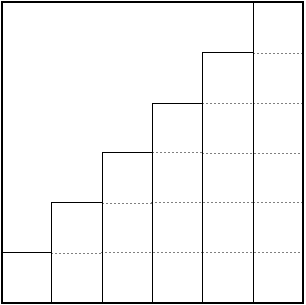
\includegraphics[scale=0.4]{FiguresMaths/SumIntegersGeometricBasis}
\caption{Representing the first $n$ integers using basic unit squares; $n=6$ in this example.}
       \label{fig:sumIntegersGeo1}
\end{center}
\end{figure}
\begin{figure}[h]
\begin{center}
       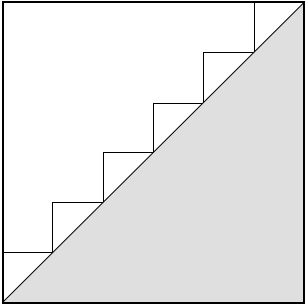
\includegraphics[scale=0.4]{FiguresMaths/SumIntegersGeometricIntermediate}
\caption{The area of the lower-right triangle (light grey) is one-half that of
  the entire $n \times n$ square.}
       \label{fig:sumIntegersGeo2}
\end{center}
\end{figure}
\begin{figure}[h]
\begin{center}
       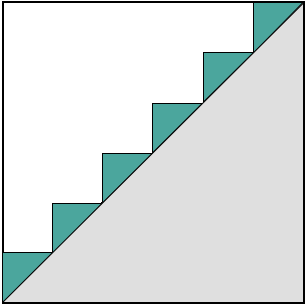
\includegraphics[scale=0.4]{FiguresMaths/SumIntegersGeometricFinal}
\caption{The area of the (dark) triangles sitting on the upper
  diagonal of the $n \times n$ square is $\frac{1}{2} n$.}
       \label{fig:sumIntegersGeo3}
\end{center}
\end{figure}
\begin{enumerate}
\item
To begin, in Fig.~\ref{fig:sumIntegersGeo1} we depict the problem of
summing the first $n$ integers as the problem of determining the area
of a surface constructed from unit-side squares.

\item
Next, we illustrate in Fig.~\ref{fig:sumIntegersGeo2} that the area of
the lower-right triangle of the $n \times n$ square---depicted in
light grey in the figure---is one-half that of the entire $n \times n$
square.

\item
Finally, we indicate in Fig.~\ref{fig:sumIntegersGeo3} that the area
of the small (dark grey in the figure) triangles that cover the upper
diagonal of the $n \times n$ square is $\frac{1}{2} n$.  This
reckoning is because there are $n$ triangle, and each has an area that
is one-half that of a unit-side square.
\end{enumerate}
We thereby reckon the area of the surface depicting the summation as

\begin{tabular}{l}
{\it One-half the area of the $n \times n$ square,
i.e., $\frac{1}{2} n^2$} \\
\hspace*{.15in} plus   \\
{\it $n$ times the area of one-half a unit-side square,
i.e., $\frac{1}{2} n$}
\end{tabular}

\noindent
We have, thus determined the value of $S_1(n)$.
\end{proof}

\medskip

We present one final proof of
Proposition~\ref{thm:sum-first-integers-Gauss}.

\begin{proof}
{\bf A combinatorial proof.}
\index{sum of first $n$ integers!a A combinatorial reckoning}
%
The following argument is {\it combinatorial} in that it achieves its
goal by {\em counting} instances of the first $n$ integers, laid out
in a line.

Place (tokens that represent) the integers $0$ to $n$ along a line.
For each integer $i$, count how many integers $j > i$ lie to its
right.  We see that in general, there is a {\it block} of $n-i$
integers that lie to the right of integer $i$.  In detail: the block
of integers lying to the right of $i=0$ contains $n$ values of $j$;
the block to the right of $i=1$ contains $n-1$ values of $j$, and so
on, as suggested in Fig.~\ref{fig:rightward-instances}.

\begin{figure}[htb]
\[
\begin{array}{lcccccc}
\mbox{All integers $\leq 4$:} &
 & 0 & 1 & 2 & 3 & 4 \\
\mbox{integers to the right of $0$:} &
 &   & 1 & 2 & 3 & 4 \\
\mbox{integers to the right of $1$:} &
 &   &   & 2 & 3 & 4 \\
\mbox{integers to the right of $2$:} &
 &   &   &   & 3 & 4 \\
\mbox{integers to the right of $3$:} &
 &   &   &   &   & 4
\end{array}
\]
\caption{A two-dimensional depiction of the right-lying
  integer-instances.}
\label{fig:rightward-instances}
\end{figure}

On the one hand, we see that the total number of right-lying integers
$j$ equals $n+(n-1)+ ... + 1 \ = \ S_1(n)$.

On the other hand, every instance of a right-lying integer can be
identified uniquely by the pair of nonnegative integers $i$ (the
instance's block) and and $j>i$ (the instance's
position-within-block).  It is not hard to verify that the total
number of right-lying integer-instances is
$\displaystyle {n+1 \choose 2}$.\footnote{We study such counting
  techniques in depth in Section~\ref{sec:counting}.}

We have thus arrived at two, perforce equal, expressions for $S_1(n)$.
\end{proof}

\medskip

Now that we know---via several arguments---the value of $S_1(n)$, we
can finally evaluate our original series in (\ref{eq:arith-seq}).
\index{arithmetic series:explicit sum}

\begin{prop}
\label{thm:sum-of-arithmetic-series}
The arithmetic series in (\ref{eq:arith-seq}) has the sum
\[
a + (a+b) + (a+2b) + (a+3b) + \cdots + (a+(n-1)b) \ = \
an + b \cdot {n \choose 2}. 
\]
\end{prop}


\paragraph{B. Perfect squares are sums of odd integers}

We now build on Proposition~\ref{thm:sum-first-integers-Gauss} to
craft {\em two} constructive proofs that each perfect square, say,
$m^2$, is the sum of the first $m$ odd integers, $1, 3, 5, \ldots,
2m-1$.  One of these proofs builds on the phenomenon of {\em finding
  invariants}.  These proofs complement the ``guess-and-verify''
inductive proof of the same result in
Proposition~\ref{thm:squares-odd-integers-induction}.

\begin{prop}
\label{thm:squares-odd-integers-Gauss}
\index{$n^2$ as sum of first $n$ odd integers}
For all $n \in \N^+$,
\begin{equation}
\label{eq:sum-of-odds}
\sum_{k=1}^n \ (2k-1)
 \ = \ 1 + 3 + 5 + \cdots + (2n-1) \ = \ n^2.
\end{equation}
That, is, the $n$th perfect square is the sum of the first $n$ odd
integers.
\end{prop}

Before presenting our two proofs of this result, we note that the
notation in (\ref{eq:sum-of-odds}) is perfectly general: every positive
odd integer $m$ can be written in the form $2n-1$ for some positive
integer $n$.

\smallskip

\begin{proof}
{\bf A textual proof.}
%
Let us adapt Gauss's ``trick'' to this problem.  Let us denote the
target sum $\sum_{k=1}^n \ (2k-1)$ by $S(n)$. 
\begin{equation}
\label{eq:add-odds}
\begin{array}{llccccccccc}
\mbox{$S_n$ ``forwards'':} &
S(n) \ = 
& 1 & + & 3 & + & \cdots & + & (2n-3) & + & (2n-1) \\
 & & & & & & & & & &  \\
\mbox{$S_n$ ``in reverse'':} &
S(n) \ =
& (2n-1) & + & (2n-3) & + & \cdots & + & 3 & + & 1
\end{array}
\end{equation}
Now add the two representations of $S(n)$ in (\ref{eq:add-odds}) {\em
  columnwise}.  Because each of the $n$ column-sums equals $2n$, we
find that
\begin{equation}
\label{eq:sum-of-odds-sum}
2 S(n) \ = \ 2 \sum_{k=1}^n \ (2k-1) \ = \ 2n^2.
\end{equation}
We thus derive the desired summation (\ref{eq:sum-of-odds}) when we
divide both sides of equation (\ref{eq:sum-of-odds-sum}) by $2$.
\end{proof}

\medskip

\begin{proof}
{\bf A proof using algebra.}
%
Our second proof derives this result, via a simple calculation, as a
corollary of Proposition~\ref{thm:sum-first-integers-Gauss}.

By direct calculation, we have
\begin{eqnarray*}
\sum_{k=1}^n \ \left( 2k-1 \right)
   & = & 2 \sum_{k=1}^n \ k \ \ - \ n \\
   & = & 2 \frac{n (n+1)}{2} \ \ - \ n \ \ \ \ \mbox{ by
  Proposition~\ref{thm:sum-first-integers-Gauss}} \\
   & = & (n^2 + n) - n \\
   & = & n^2.
\end{eqnarray*}
\end{proof}

\medskip

Our next proof is purely pictorial, with a bit of reasoning mixed in.
The only ``sophisticated'' reasoning requires knowing that
\[ (n+1)^2 \ = \ n^2 \ + \ 2n \ + \ 1. \]

\begin{proof}
{\bf A proof ``by pictures''.}
%
Our pictorial proof begins by representing an integer $n$ as a
horizontal sequence of $n$ ``bullets'', i.e., dark circles.  The
problem of summing the first $n$ odd integers then begins with a
picture such as appears in Fig.~\ref{fig:sumOdds1}, for the
illustrative case $n=5$.
\begin{figure}[h]
\begin{center}
       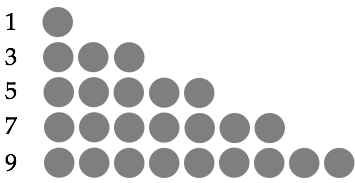
\includegraphics[scale=0.4]{FiguresMaths/SumOddsBasis}
\caption{Representing the first $n$ odd integers using bullets.  In
  this illustration, $n=5$.}
       \label{fig:sumOdds1}
\end{center}
\end{figure}

Starting with such a picture, we take each row of $2c+1$ bullets and
fold it at its midpoint so that it becomes a reversed letter $L$.  The
row of $2c+1$ bullets becomes an $L$ whose horizontal portion (at the
bottom of the reversed $L$) is a row of $c+1$ bullets and whose
vertical portion (at the right of the reversed $L$) is a column of
$c+1$ bullets.  See Fig.~\ref{fig:sumOdds2} wherein the depicted
values of $c$ are $c = 0, 1, 2, 3, 4$.
\begin{figure}[h]
\begin{center}
       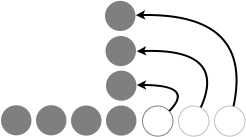
\includegraphics[scale=0.4]{FiguresMaths/SumOddsIntermediate}
              \caption{Folding a single row into a reversed letter $L$.}
       \label{fig:sumOdds2}
\end{center}
\end{figure}

Once we have folded every row of bullets into a reversed $L$, we nest
the $L$'s in the manner depicted in Fig~\ref{fig:sumOdds3}.
\begin{figure}[h]
\begin{center}
       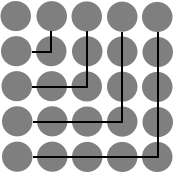
\includegraphics[scale=0.4]{FiguresMaths/SumOddsFinal}
\caption{The final picture organized as an $n \times n$ square
  array of bullets.}
       \label{fig:sumOdds3}
\end{center}
\end{figure}
Clearly, this nesting produces an $n \times n$ square array of
bullets.  
\end{proof}

\medskip

\begin{proof}
{\bf A proof by rearranging terms.}
%
We describe in Section~\ref{sec:Fubini} how the Italian mathematician
Guido Fubini
\index{Fubini, Guido}
%
was able to make notable mathematical progress by rearranging
representations \cite{Fubini}.  Within the context of the current
chapter, such rearrangements work on the terms of a summation of
interest.  Indeed, using this strategy, we obtain a surprising,
delightful proof of Proposition~\ref{thm:squares-odd-integers-Gauss}.
Let us take the odd integers in order, in groups of sizes $1$, then
$2$, then $3$, and so on.  We begin with the first $n$ odd integers in
order:
\[ 1, \ 3, \ 5, \ 7, \ 9, \ 11, \ 13, \ 15, \ 17, \ 19, \ \ldots \]
Now we start peeling off prefixes of successive numbers of odd
integers and arranging them in an array, as depicted in
Table~\ref{tab:SumOddsTriangle}.
\begin{table}[h]
\label{tab:SumOddsTriangle}
\caption{The sums of successive odd numbers and the sum of
  successive cubes}
\[
\begin{array}{llrrrrclcc}
\mbox{group of size 1:} & &
1,  &    &     &     &  \rightarrow & 1           & = & 1^3 \\
\mbox{group of size 2:} & &
3,  &  5, &     &    &  \rightarrow & 2 \times 4  & = & 2^3 \\
\mbox{group of size 3:} & &
7,  &  9, & 11, &    &  \rightarrow & 3 \times 9  & = & 3^3 \\
\mbox{group of size 4:} & &
13, & 15, & 17, & 19 &  \rightarrow & 4 \times 16 & = & 4^3 \\
\end{array}
\]
\end{table}
What we note is that---at least with the illustrated portion of the
procedure, the $k$th group, of size $k$, adds up to $k^3$.

Before we proceed further, let us verify---by induction---that this
pattern persists indefinitely.
\begin{description}
\item[{\bf Base for the induction.}]
The trivial one-term entry in row $1$ of Table~\ref{tab:SumOddsTriangle}
provides the base for our induction.

\item[{\bf Inductive hypothesis}.]
We know from Proposition~\ref{thm:sum-first-integers-Gauss} that the
$k$th group consists of $k$ consecutive odd numbers beginning with
\[ 2 {k \choose 2} -1 \ \ \ \ \
\mbox{which is the} \ \ \ \ \
\left[ {k \choose 2} +1 \right]\mbox{th odd number}
\]

\item[{\bf Inductive extension}.]
%
Since successive odd numbers differ by $2$, we know that the $k$th
group consists of the odd integers
\[
2 {k \choose 2} -1, \ 2 {k \choose 2} +1, \ 2 {k \choose 2} +3 ,
\ldots, \
2 {k \choose 2} +2k-1
\]
hence has sum
\[
2k {k \choose 2} \ - \ 2 {k \choose 2} +k
\ = \ k^3.
\]
\end{description}

{\Arny More calculation!  BOO!  Please complete this.  I seem to be
  off by 1}
With the preceding inductive verification, we have a way of computing
the first $n$ odd numbers by computing an initial 
We give another proof that tells us something more on numbers of their interactions.
We consider numbers instead of bullets, and we use a similar principle as Fubini, that is to determine a
suitable organization of the numbers and count them in a simple way.
For the concern of computing the sum of the first odd numbers, we organize them as shown in Table~\ref{tab:SumOddsTriangle}.
One number in the first row, two in the second, $k$ on the $k$th row.
There are $\Delta_p$ (complete) rows. 
The result is obtained by summing up the elements of each row.
The sum in a row is equal to the perfect cube of this row.
This result can be easily proven. 
{\Denis Should I develop here? or we can let it as an exercice?}


\medskip

Computing the sum of the first cubes can be done in a similar way as the sum of integers or the sum of squares.
This is detailed in Section~\ref{sec:sum-of-i2c}
\end{proof}

\subsection{Geometric Sums and Series}
\label{sec:geometric-sums}


\subsubsection{General development}
\label{sec:general-geometric}

We define geometric sequences and learn how to calculate their sums
via the following generic example.
\index{geometric sequence}
\index{geometric series}
\begin{equation}
\label{eq:geom-seq}
\begin{array}{l}
\mbox{An $n$-term geometric sequence:} \\
\hspace*{.25in}a, \ ab, \ ab^2, \ \ldots, ab^{n-1} \\
 \\
\mbox{The corresponding geometric series:} \\
\hspace*{.25in}a + ab + ab^2 + \cdots + ab^{n-1} \ = \
 a (1+ b + b^2 + \cdots + b^{n-1})
\end{array}
\end{equation}
It is clear just from this definition that we can sum the series in
(\ref{eq:geom-seq}) by summing just the sub-series
\begin{equation}
\label{eq:geom-series}
S_{b}(n) \ \eqdef \
1+ b + b^2 + \cdots + b^{n-1}.
\end{equation}

Along the way to developing a solution technique for the series
$S_{b}(n)$, we will uncover an even simpler solution
technique that that establsihes the following.

\begin{prop}
\label{thm:sum-infinite-geometric-series}
When $b < 1$,  the {\em infinite} series
\[ \sum_{i=0}^\infty \ b^i \ = \ 1 + b + b^2 + \cdots \]
sums to $\displaystyle \frac{1}{1-b}$.
\end{prop}

\bigskip

For general values of $b$ and general limits of summation, we have the
following slightly more cumbersome analogue of
Proposition~\ref{thm:sum-infinite-geometric-series}; that simpler
proposition follows as a corollary of the following.

\begin{prop}
\label{thm:sum-finite-geometric-series}
Let $S_{b}(n)$ be an arbitrary geometric sum, as defined in
(\ref{eq:geom-series}).

\noindent {\bf (a)}
When $b > 1$, $S_{b}(n)$ evaluates to the following sum.
\begin{equation}
\label{eq:geom-sum:b>1}
S^{b>1}_{b}(n) \ = \ \frac{b^{n}- 1}{b - 1}.
\end{equation}

\noindent {\bf (b)}
When $b < 1$, $S_{b}(n)$ evaluates to the following sum.
\begin{equation}
\label{eq:geom-sum:b<1}
S^{b<1}_{b}(n) \ = \ \frac{1 - b^n}{1-b}.
\end{equation}
\end{prop}

Of course, the uninteresting degenerate case $b=1$ sums to $n$.

\begin{proof}
{\bf A proof by textual replication.}
%
Toward the end of developing our first method for summing $S_{b}(n)$,
we note that we can rewrite the sum in two ways that are {\em
  (textually) recurrent}.

\bigskip

\noindent
{\em This phenomenon of {\em finding recurrent subexpressions} is a
  ``pattern'' of the form referred to in Section~\ref{sec:manifesto}
  as we discussed how mathematicians ``do mathematics''.  We now
  exemplify how this pattern can be exploited to find explicit sums
  for geometric series.}

\bigskip

Both of the recurrent expressions for $S_{b}(n)$ have the following form.
\begin{equation}
\label{eq:geom-series-recurrent}
S_b(n) \ = \ \alpha \cdot S_b(n) \ + \ \beta(n)
\end{equation}
where $\alpha$ is a constant and $\beta(n)$ is a function of $n$; both
$\alpha$ and $\beta(n)$ may depend on the parameter $b$.
\begin{equation}
\label{eq:geom-series-replicate}
\begin{array}{cclcl}
S_{b}(n) 
  & = &
1+ b + b^2 + \cdots + b^{n-1} & & \\
  &   &   &  & \\
  & = &
1 + b \cdot S_{b}(n) - b^n
   & = & b \cdot S_{b}(n) \ + \ (1 - b^n) \\
  &   &   &  & \\
  & = &
{\displaystyle
b^{n-1} + \frac{1}{b} \cdot S_{b}(n) - \frac{1}{b}
}
  & = &
{\displaystyle \frac{1}{b} \cdot S_{b}(n) \ + \ \frac{b^n -1}{b} 
}
\end{array}
\end{equation}
The significance of a recurrent expression of the form
(\ref{eq:geom-series-recurrent}) is that it exposes an explicit value
for $S_b(n)$:
\begin{equation}
\label{eq:geom-series-generic}
S_b(n) \ = \ \frac{\beta(n)}{1 - \alpha}
\end{equation}

We can now combine the generic value (\ref{eq:geom-series-generic}) of
$S_b(n)$ with the specialized recurrent expressions for $S_b(n)$ in
(\ref{eq:geom-series-replicate}) to derive two explicit solutions for
$S_b(n)$.
\begin{enumerate}
\item
The first solution is most useful and perspicuous when $b>1$.  In this
case, we find that
\[ \left( 1 - \frac{1}{b} \right)  S^{b>1}_{b}(n) \ = \ b^{n-1} -
\frac{1}{b}, \]
which can easily be rearranged to the equivalent and more
perspicuous form (\ref{eq:geom-sum:b>1}).

\item
The second solution is most useful and perspicuous when $b < 1$.  In this
case, we find that
\[ (1-b) S^{b<1}_{b}(n) \ = \ 1 \ - \ b^n \]
which can easily be rearranged to the equivalent and more
perspicuous form (\ref{eq:geom-sum:b<1}).
\end{enumerate}
\end{proof}

Note that both $S^{b>1}_{b}(n)$ and $S^{b<1}_{b}(n)$ have simple {\em
  approximate} values which are useful in ``back-of-the-envelope''
calculations: For very large values of $n$, we have
\begin{equation}
\label{eq:geom-sum:approx}
S^{b>1}_{b}(n) \ \approx \ \frac{b^n}{b-1} \ \ \
\mbox{while} \ \ \
S^{b<1}_{b}(n) \ \approx \ \frac{1}{1-b} .
\end{equation}
The expression for $S^{b<1}_{b}(n)$ in (\ref{eq:geom-sum:approx}) is
actually a rewording of
Proposition~\ref{thm:sum-infinite-geometric-series}.

\medskip

\begin{proof}
{\bf A pictorial proof of Proposition~\ref{thm:sum-infinite-geometric-series}.}
%
Fig.~\ref{fig:sumGeoBasis} depicts a pictorial process whose analysis
provides a rigorous argument that $\displaystyle \sum_{i=0}^\infty
\ 2^{-i}$ evaluates to $2$ (as promised by
Proposition~\ref{thm:sum-infinite-geometric-series}).
\begin{figure}[h]
\begin{center}
       \includegraphics[scale=0.4]{FiguresMaths/SumGeometric1sur2Bis}
 \caption{Arranging successive rectangles to sum $\displaystyle
   \sum_{i=0}^\infty \ 2^{-i}$.}
       \label{fig:sumGeoBasis}
\end{center}
\end{figure}
We measure fractional quantities by the portion of a unit-side
rectangle that they fill.  Thus (follow in the figure): The initial
term of $\displaystyle \sum_{i=0}^\infty \ 2^{-i}$, namely $1$, is
represented by the unit square that is labeled ``$1$'' in the figure.
The next term of the series, namely $1/2$, is represented by the
rectangle labeled ``$1/2$'' in the figure.  We proceed with
successively smaller rectangles representing successively smaller
inverse powers of $2$.  As the process proceeds, we observe
increasingly more of the righthand unit-side square being filled.  In
fact, one can argue that {\em every} point in the righthand square
eventually gets covered by some small rectangle (as $n$ tends to
$\infty$), thereby establishing that the infinite series
$\displaystyle \sum_{i=0}^\infty \ 2^{-i}$ sums to $2$.

\ignore{*******
The result is immediate while considering a basic unit square and its
successive decompositions while divided by $2$.
Thus, the whole surface corresponds to the sum of $(\frac{1}{2})^k$. 
It is equal to $2$ (surface of the two big squares) and it is completely filled. 
***********}

This procedure is hard---but not impossible---to adapt to values of $b
<1$ other than $\frac{1}{2}$.
\begin{figure}[h]
\begin{center}
       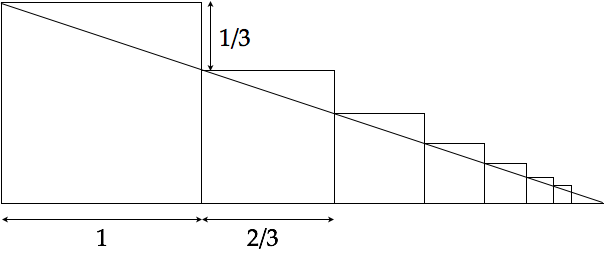
\includegraphics[scale=0.4]{FiguresMaths/SumGeometric2tiers}
\caption{Geometric series obtained by an adequate cascading of
  shrinking squares (for $b = \frac{2}{3}$).}
       \label{fig:sumGeoGeneral}
\end{center}
\end{figure}
Fig.~\ref{fig:sumGeoGeneral} suggests, for the case $b = \frac{2}{3}$
how to achieve such an adaptation for any value of $b$ with $0 \leq b
<1$, by an appropriately chosen cascade of shrinking squares.  The
length of the base of the abutting rectangles is the value of the
infinite series $\displaystyle \sum_{i=0}^\infty \ b^{-i}$.
\end{proof}

\subsubsection{An extension and an application}

\paragraph{A. On summing ``extended'' geometric series}

We now build on our sums (\ref{eq:geom-sum:b>1},
\ref{eq:geom-sum:b<1}) for geometric series to evaluate what we shall
call ``extended'' geometric series (not a standard term), \textit{i.e.}, series
of the form
\[ S_b^{(c)}(n) \ \eqdef \ \sum_{i=1}^n \ i^c b^i \]
where $c$ is an arbitrary fixed positive integer, and $b$ is an
arbitrary fixed real number.

When $c=0$, the resulting ``extended'' geometric series is just a
geometric series, which we have studied in
Section~\ref{sec:general-geometric}.  For brevity, we ignore the case
$b = 1$, which is dealt with adequately elsewhere in this chapter,
including in Section~\ref{sec:smooth-series}.  For all other values of
$b$ and $c$, our summation-solving strategy has two primary goals:
\begin{itemize}
\item
It should be {\em inductive} in parameter $c$.  That is, the strategy
should compute a sum for the series $S_b^{(c)}(n)$ in terms of earlier
discovered sums for $S_b^{(c-1)}(n)$, $S_b^{(2)}(n)$, \ldots,
$S_b^{(0)}(n) = S_b(n)$.

\item
It should rely on the recurrent-subexpression strategy which was so
effective in Section~\ref{sec:general-geometric}.
\end{itemize}
We illustrate our strategy in detail for the case $c=1$ and sketch
only briefly how it deals with larger values of $c$.  Elementary
algebraic manipulations which are suggested by the analysis in the
case $c=1$ should thereby allow the reader to deal with any value $c >
1$.

We begin to develop our strategy by noting that
\[ S_b^{(1)}(n) \ = \ \sum_{i=1}^n \ i b^i  \]
so that
\begin{equation}
\label{eq:ext-geom-c=1.1}
S_b^{(1)}(n+1) \ = \ S_b^{(1)}(n) \ + \ (n+1) b^{n+1}
\end{equation}
Reasoning somewhat differently,
\begin{eqnarray*}
S_b^{(1)}(n+1)
     & = &
\sum_{i=1}^n \ (i+1) b^{(i+1)} \ + \ b \\
     & = &
b \cdot \sum_{i=1}^n \ (i+1) b^i \ + \ b \\
     & = &
b \cdot \left(
\left(\sum_{i=1}^n \ i b^i \right)
 \ + \
\left( \sum_{i=1}^n \  b^i \right)
\right) \ + \ b \\
     & = &
b \cdot \left( S_b^{(1)}(n) \ + \ S_b^{(0)}(n) \right) \ + \ b \\
\label{eq:ext-geom-c=1.2}
    & = &
b \cdot S_b^{(1)}(n) \ + \ b \cdot \frac{b^{n+1} + b - 2}{b-1}
\end{eqnarray*}
Combining (\ref{eq:ext-geom-c=1.1}) and (\ref{eq:ext-geom-c=1.2}) we
finally obtain
\[ S_b^{(1)}(n) \ = \
\frac{1}{b-1} \cdot \left(
(n+1) \cdot b^{n+1}
  \ - \
\frac{b}{b-1} \cdot (b^{n+1} - 1)
\right)
\]

{\Arny Please correct my arithmetic!}


{\Arny We should really do the following general version.}

\[
S_b^{(c)}(n) \ = \ \sum_{i=1}^n \ i^c b^i
\]

\[
S_b^{(c+1)}(n)
 \ = \
b \ + \ 2^{c+1} b^2\ + \ 3^{c+1} b^3 \ + \ \cdots \ + \ n^{c+1} b^n
 \ = \
b \ + \ 2 b^2\ + \ 3 b^3 \ + \ \cdots \ + \ n b^n
\]




\paragraph{B. Detecting properties of integer $n$ via $n$'s base-$b$ (positional) numeral}

We now exploit our ability to sum geometric sums to illustrate a
somewhat surprising, nontrivial fact about integers that are
``encoded'' in their positional numerals.  We hope that this ``fun''
result will inspire the reader to seek kindred numeral-encoded
properties of numbers.

\begin{prop}
\label{thm:div-by-b-bar}
An integer $n$ is divisible by an integer $m$ if, and only if, $m$
divides the sum of the digits in the base-$(m+1)$ numeral for $n$.
\end{prop}

The most familiar instance of this result is phrased in terms of our
traditional use of base-$10$ (decimal) numerals. \\
{\it An integer $n$ is divisible by $9$ if, and only if, the sum of
  the digits of $n$'s base-$10$ numeral is divisible by $9$.}

\smallskip

\begin{proof}
({\it Argument for general number-base $b$}).
%
Of course, we lose no generality by focusing on numerals without
leading $0$'s, for adding leading $0$'s does not alter a numeral's sum
of digits.

To enhance legibility, let $b = m+1$, so that we are looking at the
base-$b$ numeral for $n$.  Say that
\[ n \ = \ \delta_k \cdot b^k + \delta_{k-1} \cdot b_{k-1} + \cdots +
\delta_1 \cdot b + \delta_0, \]
so that the sum of the digits of $n$'s base-$b$ numeral is
\[ s_b(n) \ \eqdef \ \delta_k + \delta_{k-1} + \cdots + \delta_1 + \delta_0. \]
We next calculate the difference $n - s_b(n)$.  We proceed as
follows, digit by digit.
\begin{equation}
\label{eq:sum-of-digits}
\begin{array}{ccccccccccc}
n & = &
\delta_k \cdot b^k & + & \delta_{k-1} \cdot b^{k-1} & + & \cdots
  & + & \delta_1 \cdot b & + & \delta_0 \\
s_b(n) & = &
\delta_k & + & \delta_{k-1} & + & \cdots & + & \delta_1 & + & \delta_0 \\
\hline
n - s_b(n) & = &
\delta_k \cdot (b^k -1) & + &
\delta_{k-1} \cdot (b^{k-1} -1) & + &
\cdots & + &
\delta_1 \cdot (b-1) & & 
\end{array}
\end{equation}

\medskip

We now revisit summation (\ref{eq:geom-sum:b>1}).  Because $b$ is a
positive integer, so that $1 + b + \cdots + b^{a-2} + b^{a-1}$ is also
a positive integer, we adduce from the summation that {\em the integer
  $b^a -1$ is divisible by $b-1$.}

We are almost home.  Look at the equation for $n - s_b(n)$ in the
system (\ref{eq:sum-of-digits}).  As we have just seen, every term on
the righthand side of that equation is divisible by $b-1$.  It follows
therefore, that the lefthand expression, $n - s_b(n)$, is also
divisible by $b-1$.  An easy calculation, which we leave to the
reader, now shows that this final fact means that $n$ is divisible by
$b-1$ if, and only if, $s_b(n)$ is.
\end{proof}


**HERE

\section{On Summing ``Smooth'' Series}
\label{sec:smooth-series}

\subsection{Approximate Sums via Integration}
\label{sec:riemann-bounds}

This section illustrates a powerful strategy for obtaining nontrivial
upper and lower bounds on the values of sum, by finding continuous {\em
  envelopes} that bound the discrete summations both above and below.
The areas under the enveloping continuous functions---which we can
calculate via integration---provide the desired bounds on the
summations.

The strategem operates as follows.  Say that we have a sum
\[ a_1 \ + \ a_2 \ + \ \cdots \ + \ a_n \]
For convenience we use a finite sum for illustration; the stratagem
often works with infinite sums also, as our specific examples
illustrate.
\begin{enumerate}
\item
Represent the summands seriatim as abutting unit-width rectangles.  
  \begin{itemize}
  \item
Our generic example has $n$ unit-width rectangles, of respective
heights $a_1$, $a_2$, \ldots, $a_n$.

  \item
In Fig.~\ref{fig:riemann-n2}, we represent the sum
\begin{figure}[htb]
\centerline{
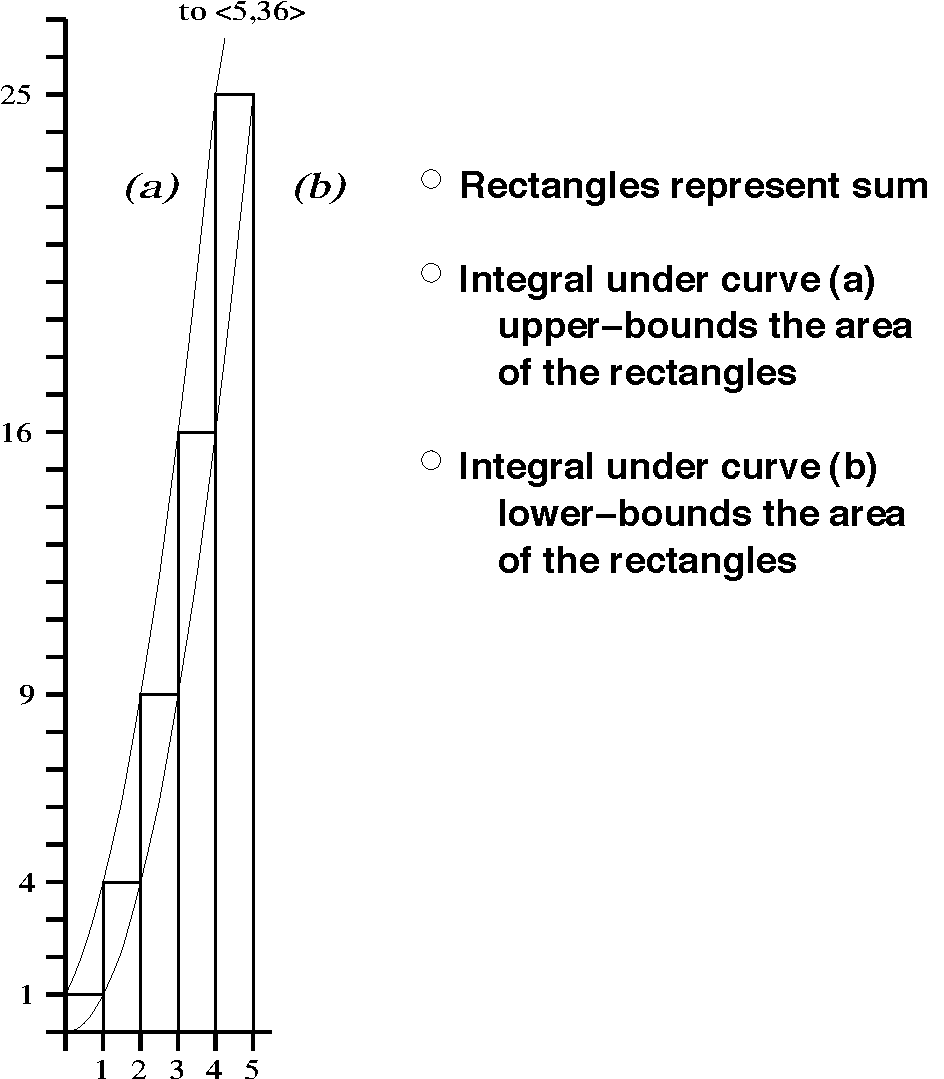
\includegraphics[scale=0.42]{riemann.pdf}
}
\caption{The summation $S_2(n) = \sum_{i=1}^n  i^2$ represented by
  the aggregate area of a sequence of unit-width rectangles, and
  bounded above an below by and ``enveloping'' pair of integrals.  The
  integral that provides the upper bound on the sum yields the area
  under the lefthand continuous curve ($a$), namely, $\int_0^n
  \ (x+1)^2 dx$.  The integral that provides the lower bound yields
  the area under the righthand continuous curve ($b$), namely,
  $\int_1^n \ x^2 dx$.}
\label{fig:riemann-n2}
\end{figure}
$S_2(n) = \sum_{i=1}^n  i^2$ using our strategem.  The rectangles
that represent the respective addends have respective heights heights
$1$, $4$, $9$, $16$, and $25$.  If we were to extend the figure
rightward (to extend the summation and encompass more addends), then
the next rectangle would have height $36$.

  \item
In Fig.~\ref{fig:riemann-harmonic}, we represent the {\em harmonic}
\begin{figure}[htb]
\centerline{
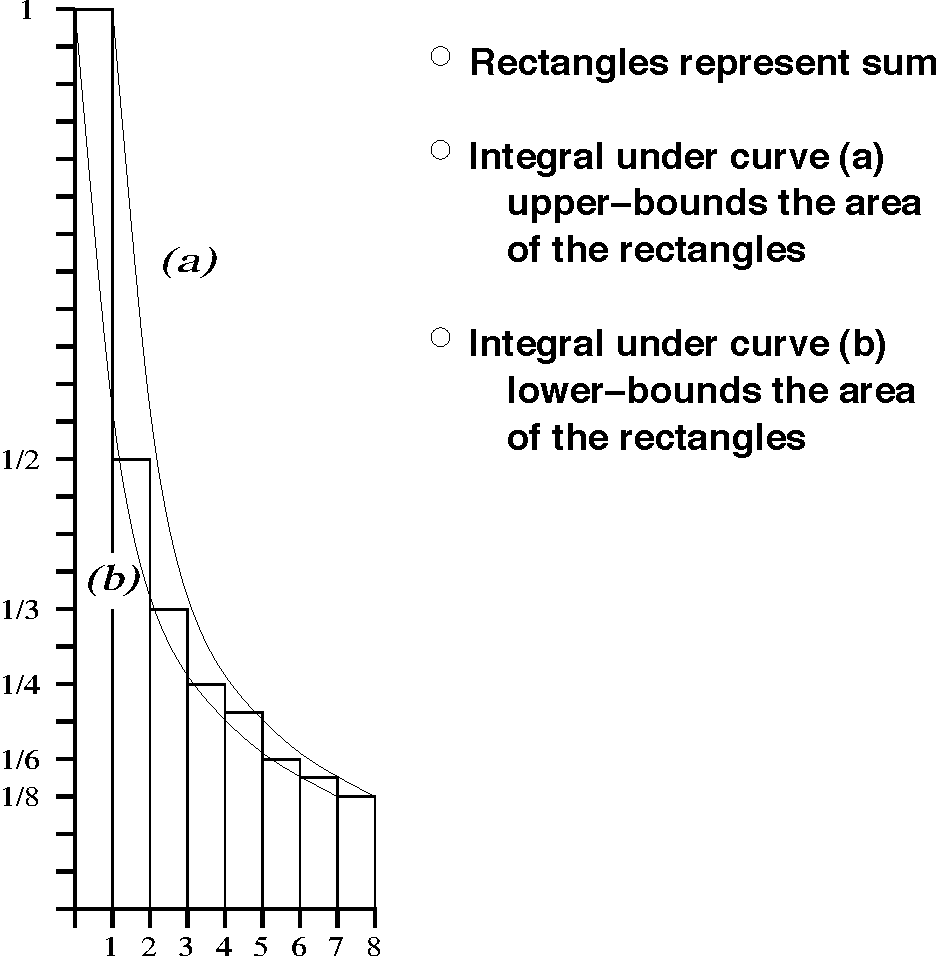
\includegraphics[scale=0.42]{riemann2.pdf}
}
\caption{The summation $S^{(H)}(n) \ = \ \sum_{i=1}^n \ 1/i$
  represented by the aggregate area of a sequence of unit-width
  rectangles, and bounded above an below by an ``enveloping'' pair of
  integrals.  The integral that provides the upper bound on the sum
  yields the area under the righthand continuous curve ($a$), namely,
  $\displaystyle \int_1^n \ \frac{1}{x} dx$.  The integral that
  provides the lower bound yields the area under the lefthand
  continuous curve ($b$), namely, $\displaystyle \int_0^{n-1}
  \ \frac{1}{x+1} dx$.}
\label{fig:riemann-harmonic}
\end{figure}
sum $S^{(H)}(n) \ = \ \sum_{i=1}^n \ 1/i$.  The rectangles that
represent the respective addends have respective heights $12$, $6$,
$4$, $3$, $16/3$, and $2$.  If we were to extend the figure rightward
(to extend the summation and encompass more addends), then the next
rectangle would have height $16/7$.
  \end{itemize}

\item
Construct a continuous curve $\overline{C}(x)$ that passes through the
upper {\em lefthand} corners of the unit-width rectangles specified by the
summation.  When constructed appropriately, the area subtended by the
abutting rectangles lies completely under this curve; hence, the area
under the continuous curve---which we obtain by integrating
$\overline{C}$---affords {\em an upper bound} on the summation of interest.

\item
Construct a continuous curve $\underline{C}(x)$ that passes through
the upper {\em righthand} corners of the unit-width rectangles
specified by the summation.  When constructed appropriately, the area
under the curve $\underline{C}(x)$ lies completely within the area
subtended by the abutting rectangles; hence, the area under the
continuous curve---which we obtain by integrating
$\underline{C}$---affords {\em a lower bound} on the summation of
interest.
\end{enumerate}

In the next three subsections, we illustrate this strategem using
summations of fixed powers of successive integers, i.e., summations of
the form $\displaystyle \sum_{i=1}^n i^c$.  In
Section~\ref{sec:sum-of-cg-1}, we focus on the case $c > -1$; in
Section~\ref{sec:sum-of-c=-1}, we focus on the case $c = -1$; in
Section~\ref{sec:sum-of-cl-1}, we focus on the case $c < -1$.


\subsubsection{Summing $c$th powers of consecutive integers: $c > -1$}
\label{sec:sum-of-cg-1}

We illustrate the technique of bounding summations via integrals by
focusing on the summations
\[ S_k(n) \ \eqdef \ \sum_{i=1}^n \ i^k, \]
for arbitrary positive integers $k$.  The technique generalizes far
beyond the summations $S_k(n)$, but this single illustration should
give the reader a firm basis from which to extrapolate to more general
summations.



We begin by describing the technique in detail for the summation
$\displaystyle S_2(n) = \sum_{i=1}^n \ i^2$.  We shall then indicate
how to extrapolate from this case to general summations $S_k(n)$.

We obtain our upper bound on $S_2(n)$ by evaluating the integral that
yields the area $\overline{A}_2(n)$ under the lefthand continuous
curve ($a$) in Fig.~\ref{fig:riemann-n2}, namely,
\begin{eqnarray}
\label{eq:upper-integral-x2}
\overline{A}_2(n) \ = \
\int_0^n \ (x+1)^2 dx & = &
  \int_0^n \ x^2 dx \ + \ 2 \int_0^n \ x dx \ + \ \int_0^n \ dx \\
\nonumber
 & = & \frac{1}{3} n^3 \ + n^2 \ + \ n \ + \ O(1).
\end{eqnarray}
We obtain our lower bound on $S_2(n)$ by evaluating the integral that
yields the area $\underline{A}_2(n)$ under the righthand continuous
curve ($b$) in the the figure, namely,
\begin{equation}
\label{eq:lower-integral-x2}
\underline{A}_2(n) \ = \
\int_1^n \ x^2 dx \ = \ \frac{1}{3} n^3 \ + \ O(1).
\end{equation}
Combining these bounds, we finally have the following two-sided bound
on $S_2(n)$.
\begin{equation}
\label{eq:bounds-sum-x2}
\frac{1}{3} n^3 \ + \ O(1)
  \ \ \leq \ \ \sum_{i=1}^n \ i^2
  \ \ \leq \ \ \frac{1}{3} n^3 \ + n^2 \ + \ n \ + \ O(1)
\end{equation}

\medskip

For summations $S_k(n)$ with $k >2$, we follow the roadmap of the case
$k=2$, invoking as a technical tool the following special case of
Newton's {\it Binomial Theorem}.\footnote{The general form of the
  Binomial Theorem expands the polynomial $(x+y)^k$ rather than
  $(x+1)^k$.}

\begin{theorem}[The Restricted Binomial Theorem]
\label{thm:restricted-binomial-thm}
For all positive integers $k$,
\[ (x+1)^k \ = \
\sum_{i=0}^k \ \ {k \choose i} x^{k-i}.
\]
\end{theorem}

\begin{quote}
As usual, the {\it binomial coefficients} are defined and denoted as
follows.
\[
{k \choose i} \ = \ \frac{k!}{i!(k-i)!} \ = \
\frac{k(k-1)(k-2) \cdots (k-i+1)}{i(i-1)(i-2) \cdots 1}
\]
\end{quote}

The extrapolation from $S_2(n)$ to general $S_k(n)$ begins with the
straightforward exercise of crafting analogues of
Fig.~\ref{fig:riemann-n2} for arbitrary summations $S_k(n)$.
Parallelling the reasoning that led us to the relations
(\ref{eq:upper-integral-x2}) and (\ref{eq:lower-integral-x2}) we
obtain:
\begin{itemize}
\item
an upper bound on summation $S_k(n)$ by evaluating the integral that
yields the area $\overline{A}_k(n)$ under the continuous curve that
passes through the upper lefthand corners of the unit-width rectangles
specified by summation $S_k(n)$.
\begin{eqnarray}
\label{eq:upper-integral-xk}
\overline{A}_k(n) \ = \
\int_0^n \ (x+1)^k dx & = &
\int_0^n \ \left(
\sum_{i=0}^k \ \ {k \choose i} x^{k-i} \right) dx \\
\nonumber
  & = &
\sum_{i=0}^k \ \ \frac{1}{k-i+1} {k \choose i} n^{k-i+1} \ + \ O(1)
\end{eqnarray}
This is a proper upper bound because the region defined by this curve
totally contains the region subtended by the rectangles.

\item
a lower bound on summation $S_k(n)$ by evaluating the integral that
yields the area $\underline{A}_k(n)$ under the continuous curve that
passes through the upper righthand corners of the unit-width
rectangles specified by summation $S_k(n)$.
\begin{equation}
\label{eq:lower-integral-xk}
\underline{A}_k(n) \ = \ 
\int_1^n \ x^k dx \ = \ \frac{1}{k+1} n^{k+1} \ + \ O(1).
\end{equation}
This is a proper lower bound because the region subtended by the
rectangles totally contains the below this curve
\end{itemize}

\noindent
Using this strategy, one finds that for any positive integer $k$,
summation $S_k(n)$ enjoys the following two-sided bound:
\begin{equation}
\label{eq:bounds-sum-xk}
\frac{1}{k+1} n^{k+1} \ + \ O(1)
  \ \ \leq \ \ \sum_{i=1}^n \ i^k
  \ \ \leq \ \ 
\sum_{i=0}^k \ \ \frac{1}{k-i+1} {k \choose i} n^{k-i+1} \ + \ O(1)
\end{equation}
It follows that $S_k(n)$ enjoys the following asymptotic behavior.
\begin{equation}
\label{eq:behavior-sum-xk}
S_k(n) \ = \
\sum_{i=1}^n \ i^k \ \approx \ \frac{1}{k+1} \ n^{k+1}.
\end{equation}

\medskip

We now discuss how to ``expand'' bounds such as
(\ref{eq:bounds-sum-xk}) into explicit expressions for the summations
$S_k(n)$.


\subsubsection{Summing $c$th powers of consecutive integers: $c = -1$}
\label{sec:sum-of-c=-1}

{\Arny TO BE DONE}

The {\it harmonic series} and its finite prefixes are the following
summations.
\begin{equation}
\label{eq:harmonic}
\begin{array}{lcll}
S^{(H)} & = & {\displaystyle \sum_{i=1}^\infty \ \frac{1}{i}} & \hspace*{.25in}
  \mbox{the full harmonic series} \\
S_n^{(H)} & = & {\displaystyle \sum_{i=1}^n \ \frac{1}{i} } & \hspace*{.25in}
  \mbox{the $n$-term harmonic summation} \\
\end{array}
\end{equation}

\subsubsection{Summing $c$th powers of consecutive integers: $c < -1$}
\label{sec:sum-of-cl-1}

{\Arny TO BE DONE}





\subsection{Refining approximate sums via {\em undetermined coefficients}}
\label{sec:undetermined-coefficients}
\index{method of undetermined coefficients}

We now introduce the {\em Method of Undetermined Coefficients}, a tool
that can sometimes refine approximations to summations to exact
explicit expressions.  We illustrate the tool on the summations
$S_k(n)$ that we studied in Section~\ref{sec:riemann-bounds}; we use
the tool to convert bounds on the $S_k(n)$, such as
(\ref{eq:behavior-sum-xk}), to explicit expressions for the
summations.

We illustrate the method by deriving explicit expressions for two
rather simple summations: the sum $S_1(n)$ of the first $n$ positive
integers and the sum $S_2(n)$ of the first $n$ perfect squares.

\paragraph{A. An explicit expression for $S_1(n)$}

Of course, we have already determined $S_1(n)$ in
Section~\ref{sec:arithmetic-series}, by other means.  We provide this
alternative derivation as a gentle introduction to the method of
undetermined coefficients.

\begin{prop}
{\em For all} $n \in \N$,
\[
S_1(n) \ \eqdef \ \sum_{i=1}^n \ i^2 
 \ = \  1 + 2 + \cdots + n
 \ = \  \frac{1}{2} n^2 \ + \ \frac{1}{2} n
\]
\end{prop}

\begin{proof}
We can reason from the case $k=1$ of (\ref{eq:bounds-sum-xk}) that
\[ S_1(n) \ = \ \frac{1}{2} n^2 \ + \ cn \]
for some positive constant $c$, the eponymous {\it undetermined
  coefficient} for this case.  We can discover the value of $c$ by
evaluating $S_1(n)$ at the value $n =1$.  Any value of $n$ will work;
using the {\em smallest} one simplifies our calculation.

Because $S_1(1) = 1$, we
have
\[ S_1(1) \ = \ 1 \ = \ \frac{1}{2} \ + \ c, \]
so that $c = 1/2$; in other words,
\[ S_1(n) \ = \ \frac{1}{2} \left( n^2 + n \right) \ = \ 
\frac{n(n+1)}{2}.
\]
\end{proof}
We verify this expression by induction in
Proposition~\ref{thm:sum-1-to-n-induction}.

\paragraph{B. An explicit expression for $S_2(n)$}

A modestly more complicated undetermined-coefficient calculation
allows us to evaluate the sum $S_2(n)$ of the first $n$ squares.

\begin{prop}
{\em For all} $n \in \N$,
\begin{equation}
\label{eq:sum-1-to-nsq}
S_2(n) \ \eqdef \ \sum_{i=1}^n \ i^2 
 \ \eqdef \  1 + 4 + \cdots + (n-1)^2 + n^2
 \ = \ \frac{1}{3} n^3 \ + \ \frac{1}{2} n^2 \ + \ \frac{1}{6} n
\end{equation}
\end{prop}

$S_2(n)$ is often expressed in a more aesthetic form:
\[ S_2(n) \ = \
\frac{1}{6} n (n+1)(2n+1) \ = \
\frac{2n+1}{3} \cdot {n \choose 2}.
\]

\begin{proof}
We can reason from the case $k=2$ of (\ref{eq:bounds-sum-xk}) that
\begin{equation}
\label{eq:symbolic-cubic}
\sum_{i=0}^n \ k^2 \ = \ \frac{1}{3} n^3 + c_2 n^2 + c_1 n.
\end{equation}
for some positive numbers $c_2$ and $c_1$, the eponymous {\it
  undetermined coefficient} for this case.

We begin our determination of the constants $c_1$ and $c_2$ by
instantiating the polynomial in (\ref{eq:symbolic-cubic}) with the
smallest two values of $n$, namely, $n = 1,2$.  Of course, any two
values will work, but using the {\em smallest} ones simplifies
calculations.  These instantiations leave us with the following pair
of linear equations.
\[
\begin{array}{cccccl}
n=1: & \sum_{i=0}^1 \ k^2
   & = & 1 & = &
1/3 \ + \ c_2 \ + \ c_1 \\
n=2: & \sum_{i=0}^2 \ k^2
   & = & 5 & = &
8/3 \ + \ 4 c_2 \ + \ 2 c_1
\end{array}
\]
By elementary arithmetic, these equations simplify to yield the pair
\[
\begin{array}{ccc}
c_2 \ + \ c_1   & = & 2/3 \\
2 c_2 \ + \ c_1 & = & 7/6
\end{array}
\]
These equations reveal that
\[ 2/3 \ - \ c_2 \ = \ 7/6 \ - \ 2 c_2 \]
so that 
\[ c_2 \ = \ 1/2 \]
which means that
\[ c_1 \ = \ 1/6. \]
We have, thus, derived equation~(\ref{eq:sum-1-to-nsq}).  
\end{proof}

With more (calculational) work, but no new (mathematical) ideas, one
can derive explicit expressions for the sum of the first $n$ $k$th
powers, i.e., the quantity $S^{(k)}_n$, for any positive integer $k$.



\subsection{Validating Approximate Sums via Induction}
\label{sec:Sums-Induction}


We illustrate the proof technique of (Finite) Induction by proving the
correctness of two familiar summation formulas: (1) the sum of the
first $n$ positive integers and (2) the sum of the first $n$ odd
positive integers.


\begin{center}
\label{thm:sum-1-to-n-induction}
For all $n \in \N$,
\begin{eqnarray}
\nonumber
S_n \ \eqdef \ \sum_{i=1}^n \ i
 & \eqdef &
 1 + 2 + \cdots + (n-1) + n \\
\label{eq:sum-first-n}
 & = & {1 \over 2} n (n+1)
%\nonumber
% & = & {{n+1}  \choose 2}.
\end{eqnarray}
\end{center}

\begin{proof}
For every positive integer $m$, let {\bf P}$(m)$ be the proposition
\[  1 + 2 + \cdot + m \ = \ {{m+1} \choose 2}. \]
Let us proceed according to the standard format of an inductive
argument.

{\bf 1.} Because ${\displaystyle {2 \choose 2}} = 1$, proposition {\bf
  P}$(1)$ is true.

{\bf 2.} Let us assume, for the sake of induction, that proposition
{\bf P}$(m)$ is true for all positive integers strictly smaller than
$n$.  In particular, then, {\bf P}$(n-1)$ is true.

{\bf 3.} Consider now the summation
\[ 1 + 2 + \cdots + (n-1) + n. \]
Because {\bf P}$(n-1)$ is true, we know that
\[ 1 + 2 + \cdots + (n-1) \ = \ {n \choose 2}.  \]
By direct calculation, we see that
\begin{eqnarray*}
{n \choose 2} + n
  & = & \frac{n(n-1)}{2}  \ + \ n \\ 
  & = & \frac{n^2 - n + 2n}{2} \\
  & = & \frac{n^2 + n}{2} \\
  & = & {{n+1} \choose 2}
\end{eqnarray*}

Because $n$ is an arbitrary positive integer, we conclude that
{\bf P}$(n)$ is true whenever
\begin{itemize}
\item
{\bf P}$(1)$ is true
\item
{\em and}
{\bf P}$(m)$ is true for all $m < n$.
\end{itemize}
By the Principle of (Finite) Induction, then, we conclude that {\bf
  P}$(n)$ is true for all $n \in \N^+$.

\end{proof}

\bigskip

We turn now to our second summation, which asserts that each perfect
square of a positive integer, say, $n^2$, is the sum of the first $n$
odd integers, $1, 3, 5, \ldots, 2n-1$.  This proof complements the
constructive proofs of the same result in
Proposition~\ref{thm:squares-odd-integers-Gauss}.

\begin{center}
\label{thm:squares-odd-integers-induction}
For all $n \in \N^+$,
\[
\sum_{k=1}^n \ (2k-1)
 \ = \ 1 + 3 + 5 + \cdots + (2n-1) \ = \ n^2.
\]
That, is, the $n$th perfect square is the sum of the first $n$ odd
integers.
\end{center}

\noindent {\em Verification.}
%
For every positive integer $m$, let {\bf P}$(m)$ be the proposition
\[ m^2 \ = \ 1 + 3 + 5 + \cdots + 2m-1. \]
Let us proceed according to the standard format of an inductive
argument.

{\bf 1.} Because $1 \cdot 1 = 1$, proposition {\bf P}$(1)$ is true.

{\bf 2.} Let us assume, for the sake of induction, that proposition
{\bf P}$(m)$ is true for all positive integers strictly smaller than
$n$.  In particular, then, {\bf P}$(n-1)$ is true.

{\bf 3.} Consider now the summation
\[ 1 + 3 + 5 + \cdots + 2n-3 + 2n-1 \]
Because {\bf P}$(n-1)$ is true, we know that
\[ 1 + 3 + 5 + \cdots + 2n-3 + 2n-1 \ = \ (n-1)^2 + 2n-1.  \]
By direct calculation, we see that
\[ (n-1)^2 + 2n-1 \ = \ (n^2 -2n +1) + (2n-1) \ = \ n^2. \]
Because $n$ is an arbitrary positive integer, we conclude that
{\bf P}$(n)$ is true whenever
\begin{itemize}
\item
{\bf P}$(1)$ is true
\item
{\em and}
{\bf P}$(m)$ is true for all $m < n$.
\end{itemize}
By the Principle of (Finite) Induction, then, we conclude that {\bf
  P}$(n)$ is true for all $n \in \N^+$.
\qed


\ignore{********************
\subsection{Deriving and Solving Linear Recurrences}
\label{sec:linear-recurrences-2}

We have discussed already discussed the use of linear recurrences in
Section~%PLACE REFERENCE TO \ref{sec:linear-recurrences-1}.
 We now derive the mathematics
underlying this important topic.

By the time the reader has reached this paragraph, she has the
mathematical tools necessary to prove and apply what is called {\it
  The Master Theorem for Linear Recurrences} \cite{CLRS}.  This level
of mathematical preparation should be adequate for most
early-undergrad courses on data structures and algorithms, as well for
for analyzing a large fraction of the algorithms that she is likely to
encounter in daily activities.

\noindent {\bf Theorem}[The Master Theorem for Linear Recurrences]
\label{thm:master-thm}
%\index{The Master Theorem for Linear Recurrences}
{\it 
Let the function $F$ be specified by the following linear recurrence.}
\begin{equation}
\label{eq:Lin-Recur:start}
F(n) \ = \ \left\{
\begin{array}{cl}
a F(n/b) + c & \mbox{for } n \geq b \\
c & \mbox{for } n < b
\end{array}
\right.
\end{equation}
{\it
Then the value of $F$ on any argument $n$ is given by}
\begin{equation}
\label{eq:Lin-Recur:solve}
\begin{array}{lclll}
F(n) & = & (1 + \log_b n)c &  & \mbox{if } a=1 \\
     &   &                 &  & \\
     & = &
  {\displaystyle
  \frac{1-a^{\log_b n}}{1-a} \ \approx \ \frac{1}{1-a}
  }
 &  & \mbox{if } a<1 \\
    &   &                  & & \\
    & = &
  {\displaystyle
\frac{a^{\log_b n} -1}{a-1}
  }
 & & \mbox{if } a>1
\end{array}
\end{equation}


\begin{proof}
In order to discern the recurring pattern in
(\ref{eq:Lin-Recur:start}), let us begin to ``expand'' the specified
computation by replacing occurrences of $F(\bullet)$ as mandated in
(\ref{eq:Lin-Recur:start}).
\begin{equation}
\label{eq:Lin-Recur:expand}
\begin{array}{lcccc}
F(n) & = & a F(n/b) + c & & \\
     & = & a \left( a F(n/b^2) + c \right) + c
             & = & a^2 F(n/b^2) + (1 + a)c \\
     & = & a^2 \left( a F(n/b^3) + c \right) + (1+a)c
             & = & a^3 F(n/b^3) + (1 + a + a^2)c \\
     &   & \vdots & & \vdots \\
     & = & 
{\displaystyle
\left( 1 + a + a^2 + \cdots + a^{\log_b n} \right) c
} & &
\end{array}
\end{equation}
The segment of (\ref{eq:Lin-Recur:expand}) ``hidden'' by the vertical
dots betokens an induction that is left to the reader.  Equations
(\ref{eq:geom-sum:b>1}) and (\ref{eq:geom-sum:b<1}) now enable us to
demonstrate that (\ref{eq:Lin-Recur:solve}) is the case-structured
solution to (\ref{eq:Lin-Recur:start}).
\end{proof}
********************}

